\documentclass{article}
\usepackage{tikz, comment}
\usepackage{pifont}
\usepackage{fontspec, pgfplots}
\usetikzlibrary{arrows, decorations.markings, decorations.pathreplacing}
\begin{comment}
:Title: Not defined yet
:Tags: properties of equality, equation rules;absolute value rules;proper subset;equivalence properties of equality;inequality rules
:Prob: 0.778;0.7248;0.6578;0.6543;0.6069
:Author: Prof.Hu Ji-shan, HKUST
:Slug: No name yet

Description Here.........
\end{comment}
\begin{document}\centering 

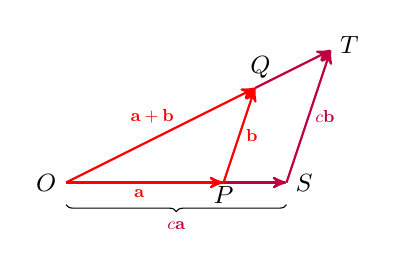
\begin{tikzpicture}[>=latex,xscale=.5*4, yscale=.5*4][font=\sf\small] 

\draw[purple, thick, ->, >=stealth'] (0, 0)node[black, left] {$O$} -- ({1.4}, {0});

\draw [decoration={brace,raise=8, mirror},decorate, xshift=0] 
(0, 0) -- ({1.4}, {0})node[purple, below, fill=white, midway, pos=0.5, xshift=0, yshift=-12, scale=0.7]{$c{\bf a}$}node[black, right]{$S$};

\draw[red, thick, opacity=1, ->, >=stealth'] (0, 0) -- (1, 0)node[opacity=1, below, midway, pos=0.5, xshift=-2, yshift=0, scale=0.7]{${\bf a}$}node[black, below, yshift=2]{$P$};

\draw[red, thick, opacity=1, ->, >=stealth'] (1, 0) -- (1.2, 0.6)node[opacity=1, right, midway, pos=0.5, xshift=0, yshift=0, scale=0.7]{${\bf b}$};

\draw[red, thick, opacity=1, ->, >=stealth'] (0, 0) -- (1.2, 0.6)node[opacity=1, above, midway, pos=0.5, xshift=-3, yshift=2, scale=0.7]{${\bf a+b}$}node[black, above, xshift=2]{$Q$};

\draw[purple, thick, opacity=1, ->, >=stealth'] (1.2, 0.6) -- ({1.2*1.4}, {0.6*1.4})node[black, right, yshift=2]{$T$};

\draw[purple, thick, ->, >=stealth'] (1.4, 0) -- ({1.4+0.2*1.4}, {0+0.6*1.4})node[opacity=1, right, midway, pos=0.5, xshift=0, yshift=0, scale=0.7]{$c{\bf b}$};

\end{tikzpicture}
\end{document}